\chapter{System Architecture}

\section{Hardware System Architecture}
\label{sec:hardware_architecture}

The system architecture is built upon an embedded platform comprising three main components: the ESP32 microcontroller unit, an external A7670G cellular modem and a host PC. This design defines the functional relationships among these hardware components.

The complete system's functional links, including power and communication pathways, are summarized in Table \ref{tab:arch_links} for clarity.

\begin{table}[H]
    \centering
    \caption{Summary of Functional Links and Communication Protocols}
    \label{tab:arch_links}
    \renewcommand{\arraystretch}{1.2}
    \begin{tabular}{>{\raggedright\arraybackslash}p{4cm} 
                    >{\raggedright\arraybackslash}p{2cm} 
                    >{\raggedright\arraybackslash}p{6.5cm}}
        \hline
        Functional Link & Protocol/Type & Purpose and Signals Transferred \\
        \hline
        Host PC $\rightarrow$ ESP32 & UART & Shell Commands: Input from the user (via terminal) to the ESP32 for interactive control and testing. \\
        \hline
        ESP32 $\rightarrow$ Host PC & UART & Console Output: Output stream carrying debug, kernel, and application status messages for monitoring. \\
        \hline
        ESP32 $\rightarrow$ A7670G & UART & AT Commands (Control): The host MPU sends high-level commands to control the modem's internal TCP/IP stack (e.g., connect, configuration). \\
        \hline
        A7670G $\rightarrow$ ESP32 & UART & AT Responses, URCs (Feedback): Returns the modem's feedback (OK, ERROR), Unsolicited Response Codes (URCs), and the received IP Data Payload. \\
        \hline
        ESP32 $\rightarrow$ A7670G & GPIO & PEN Control: Dedicated control line used to programmatically assert a hardware reset on the A7670G modem. \\
        \hline
        ESP32 Power Supply $\rightarrow$ ESP32 & DC Supply & 5V DC Supply: Provides operational power for the host MPU and its integrated Wi-Fi module. \\
        \hline
        A7670G Power Supply $\rightarrow$ A7670G & DC Supply & 5V DC Supply (2A Peak): High-capacity power line required to maintain voltage stability during the modem's high-current GSM transmission bursts. \\
        \hline
    \end{tabular}
\end{table} 

\begin{figure}[H]
    \centering
    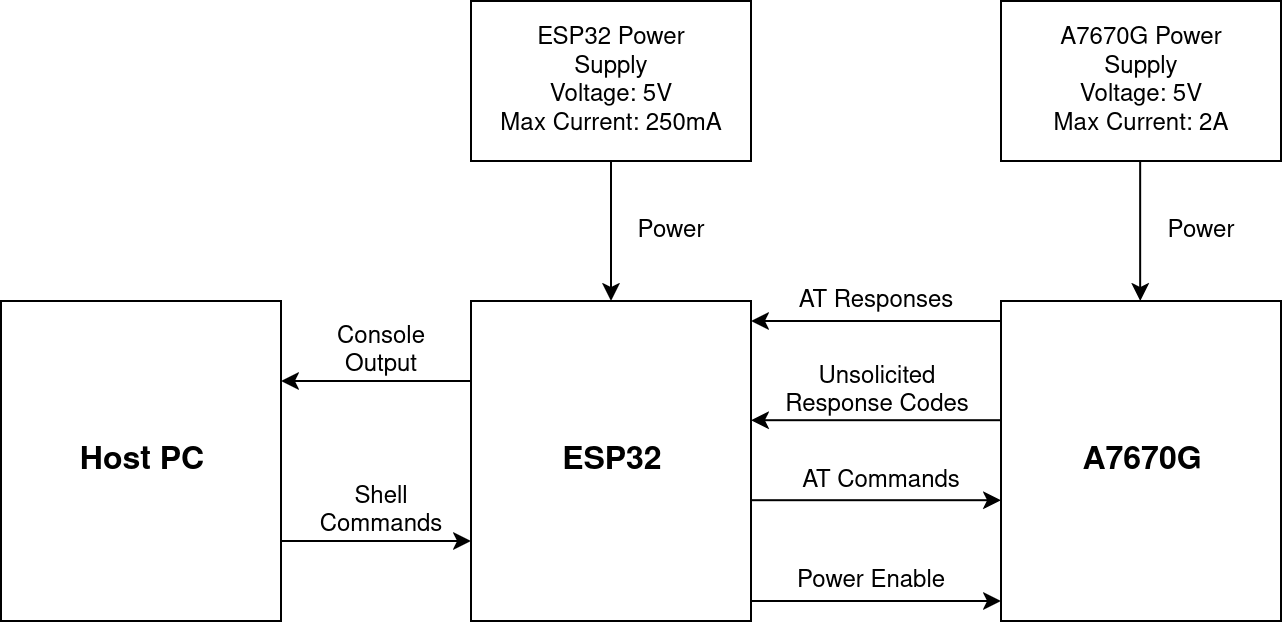
\includegraphics[width=0.85\textwidth]{"images/hardware-architecture.png"}
    \caption{Conceptual Hardware System Block Diagram. The figure illustrates the external connections and the functional relationship between the host ESP32 MPU and the external A7670G cellular modem.}
    \label{fig:hardware-arch-diagram}
\end{figure}

\section{Software Architecture}
\label{sec:software_architecture}

The software architecture is defined by the strategic layering of custom and native components within the \text{Zephyr RTOS}. The core innovation is the Adaptive Sockets Layer, designed to provide a single, resilient networking interface to the application by dynamically managing two fundamentally different network paths.

\subsection{Background: Key Zephyr Networking Abstractions}
\label{ssec:background_zephyr}

The project relies on specific networking abstractions provided by the Zephyr RTOS. Understanding the roles of these core components and the available networking paradigms is essential for interpreting the architectural diagrams:

\begin{itemize}
    \item \textbf{Sockets API:} This is the highest software layer, providing the standard POSIX-like functions (\texttt{connect}, \texttt{send}, \texttt{recv}, ...) used by application code to request network services.
    \item \textbf{Network Context (\texttt{net\_context}):} This data structure represents the state of a single network session (e.g., a TCP connection). In the native networking stack, every socket created by the application is assigned a unique Network Context.
    \item \textbf{Network Interface (\texttt{net\_if}):} A logical structure that represents a path to a specific network medium. Each physical network device has only one \texttt{net\_if} allocated at compile time.
\end{itemize}

\subsubsection{Data Handling in the Native Zephyr Stack}
When the Sockets API receives application data, it passes that data, along with the session's Network Context, to the lower layers. The data is handled by the \texttt{net\_if} for protocol processing. The Zephyr stack then performs the necessary protocol work—such as adding IP and TCP headers—before handing the network packet off to the Device Drivers, which transmit the data to the physical hardware. While the \texttt{net\_if} structure is created at compile time, network contexts are created during runtime and bound to network interfaces.

\subsection{Zephyr Networking Implementation Paradigms}
\label{ssec:networking_paradigms}
Zephyr offers flexibility in networking implementation, allowing developers to choose which protocol layers are handled by the microprocessor versus which are delegated (offloaded).

\begin{enumerate}
    \item \textbf{Native Full Stack Implementation (Standard):} The developer implements the low-level Device Driver to communicate with the L2 (Data Link) Layer. This provides very little control to the developer but allows Zephyr to automatically handle the full stack, including TCP/IP and the Sockets API. This is the path used by the Wi-Fi interface.
    \item \textbf{Network Offloading (Partial Control):} The developer implements a driver that presents a specific API used by the \texttt{net\_if}. This implementation allows the driver to bypass the L2 layer of \text{Zephyr's} native networking stack. This provides increased control over the network path but still relies on Zephyr for the higher layers (Net Contexts and Sockets).
    \item \textbf{Sockets Offloading (Full Control):} The developer implements the Sockets API and all layers below. This method provides the greatest degree of control over network behavior—a necessity for implementing dynamic routing—but makes the developer responsible for the full stack. This paradigm is typically used to integrate external hardware that executes the entire TCP/IP and Sockets stack internally. The Adaptive Sockets Layer is built atop this framework specifically to leverage this full control aspect for implementing transparent failover.
\end{enumerate}

\subsection{Software Architecture: Layer-by-Layer Implementation}
\label{ssec:software_implementation}

The architecture is built on a custom separation of management and session-handling logic. For definitions of the fundamental Zephyr networking terms used below (e.g., Network Context and $\texttt{net\_if}$), please refer to Section \ref{ssec:background_zephyr}. The structure is best understood by examining the system layer by layer, as illustrated in Figure \ref{fig:software-arch}.

\begin{figure}[H]
    \centering
    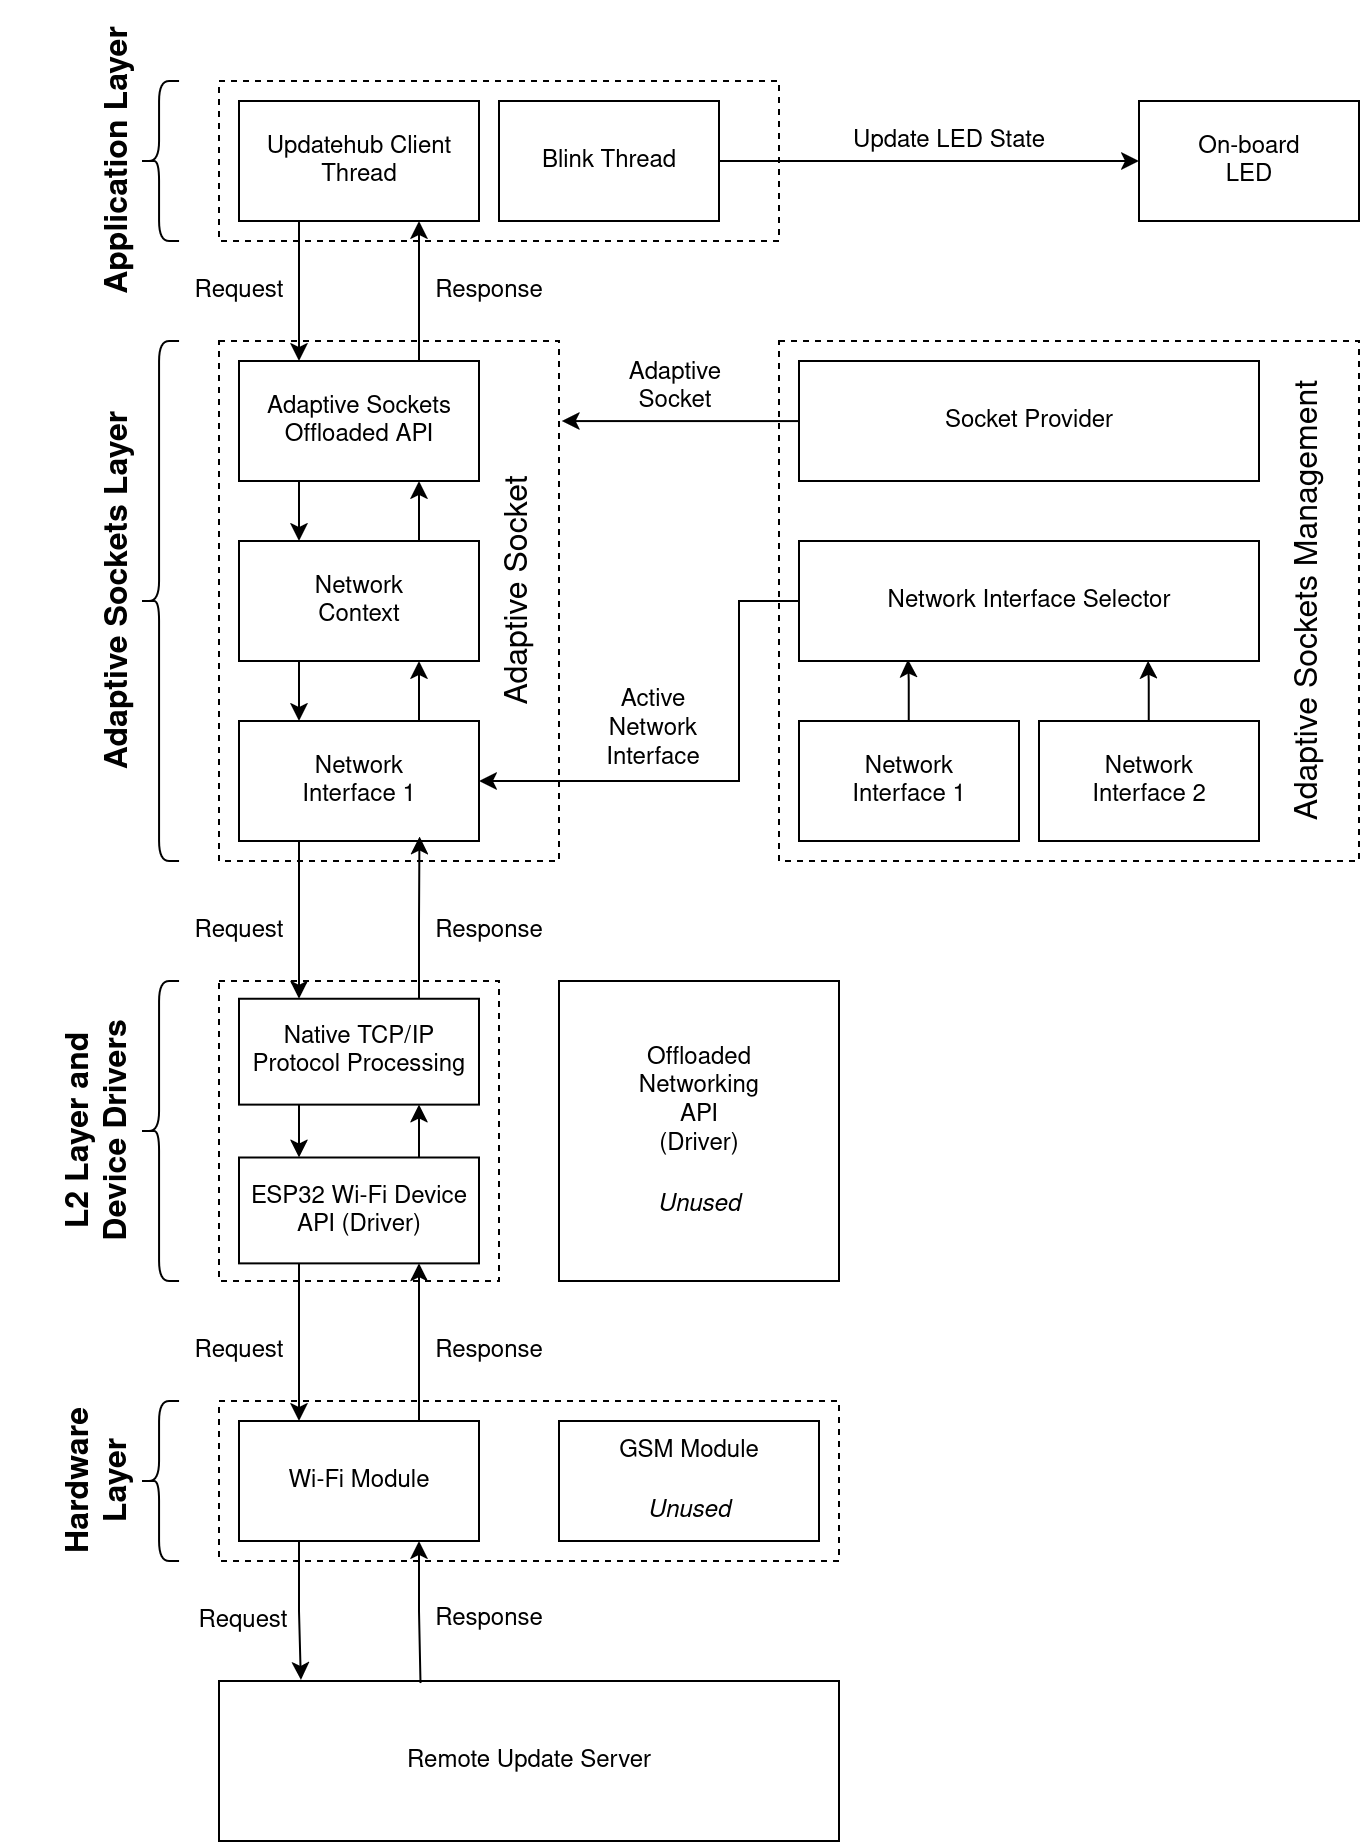
\includegraphics[width=0.95\textwidth]{"images/software-architecture.png"}
    \caption{Conceptual Software Architecture illustrating the data path of a single Adaptive Socket Instance. The diagram highlights the functional split between the Native Wi-Fi and Offloaded GSM network stacks.}
    \label{fig:software-arch}
\end{figure}

\subsubsection{Layer 1: Application Layer}
\label{sssec:application_layer}

The Application Layer sits at the highest level and contains the primary application threads that interact with the system. While the \text{Zephyr RTOS} manages numerous internal system threads for kernel operations, the following are the primary threads created and managed by the application:

\begin{itemize}
    \item \textbf{UpdateHub Client Thread:} The main application thread, which polls the \text{FOTA} server by making \textbf{Sockets API Calls} (e.g., \texttt{connect}, \texttt{send}, ...). This thread is responsible for initiating all network transactions.
    \item \textbf{Blink LED Thread:} A non-networking thread providing visual confirmation of system activity. Its blinking frequency is utilized to communicate system state: the frequency will change from a slow, steady rate to a rapid rate to confirm that a FOTA update has occurred successfully.
\end{itemize}

\subsubsection{Layer 2: Adaptive Sockets Layer (Custom Abstraction)}
\label{sssec:adaptive_sockets_layer}

The Adaptive Sockets Layer is the core innovation, providing a flexible and resilient Sockets API to the application. It is designed to be well decoupled from the physical network technologies, though for this project, it manages the Wi-Fi interface as the primary link and the GSM interface as the secondary. This layer is split into two primary functional components:

\paragraph{Adaptive Socket (The Router)}
This is the session-specific structure returned to the application. The primary logic to switch networks is embedded within the socket itself, allowing it to perform dynamic failover checks on every operation.

\begin{itemize}
    \item \textbf{Adaptive Sockets Offloaded API:} The API entry point for the session. Because the Adaptive Sockets implementation is registered as the highest priority sockets API provider in Zephyr, the operating system routes the application's generic Sockets API Calls directly to the Adaptive Sockets Layer.
    \item \textbf{Network Context:} The singular session state data structure. It is contained within the socket instance and is the element that gets re-bound to a different $\texttt{net\_if}$ during failover.
    \item \textbf{Network Interface Reference ($\texttt{net\_if}$):} A pointer to the currently assigned Network Interface (Wi-Fi or GSM).
\end{itemize}

\paragraph{Adaptive Sockets Management (The Manager)}
The Layer acts as the central policy manager and resource provider, holding the following helpers and resources:

\begin{itemize}
    \item \textbf{Network Interface References ($\texttt{net\_if\_1}$ and $\texttt{net\_if\_2}$):} Holds static references to the two possible network interfaces.
    \item \textbf{Operational Status Fields:} Internal flags updated by the Monitoring Thread that track the current viability and stability of the underlying network links.
    \item \textbf{Network Interface Selector (Helper):} A helper function that reads the $\text{Operational Status Fields}$ to determine the optimal $\texttt{net\_if}$ reference at a given moment (e.g., for initial setup).
    \item \textbf{Socket Factory (Provider):} The \texttt{get} socket function, which returns a newly created Adaptive Socket. It uses the Network Interface Selector to perform the initial route binding.
\end{itemize}

\subsubsection{Layer 3: L2 Layer and Drivers}
\label{sssec:l2_drivers}

This layer dictates the protocol processing required for each path, clearly contrasting the host-processed Wi-Fi stack with the modem-processed GSM stack. The difference is critical, as the Adaptive Sockets Layer must manage sessions across these two fundamentally different network paradigms.

\paragraph{Common Interface}
Crucially, despite their radically different internal processing mechanisms, both the Wi-Fi and GSM drivers implement the Zephyr Net Device API. This standard API exposes an identical interface to the higher layers (Net interface and Net Context). This uniformity is precisely what allows the Adaptive Sockets Layer to route network requests and responses through both paths interchangeably, as it sees two identical communication channels above the driver level.

\paragraph{Native Wi-Fi Route}
For the Wi-Fi path, the system uses the full Native Network Stack. The ESP32 Wi-Fi driver provided by Zephyr is utilized. This driver is a Native Stack Driver that exposes the Net Device API to the L2 (Data Link) layer of the host operating system. This means that the Native TCP/IP Protocol Processing—where the microprocessor executes all IP, TCP, UDP, and L2 protocol logic—must occur on the ESP32.

\paragraph{Offloaded GSM Route}
The GSM path utilizes a custom Network Offloaded Driver to communicate with the external A7670G modem via UART. This approach implements the Network Offloading paradigm (refer to Section \ref{ssec:networking_paradigms}), where the \texttt{net\_if} is configured to allow the driver to bypass the L2 layer of the host's native networking stack. Instead, the Offloaded Driver uses AT Commands to relay data and control to the modem, which handles all L2 protocol processing and packet framing internally. This reduces the computational and memory load on the host microprocessor but introduces the complexity of managing the external modem's command interface.

\subsubsection{Layer 4: Hardware Layer}
\label{sssec:hardware_layer}

This layer includes the physical components that perform the actual transmission and reception of network data:

\begin{itemize}
    \item \textbf{Built-in Wi-Fi Module:} The $\text{ESP32}$'s integrated radio system, managed by the Native Stack Driver, which handles all communication over the Wi-Fi medium.
    \item \textbf{A7670G Cellular Modem:} The external module, managed by the Offloaded Driver, which executes the entire cellular $TCP/IP$ stack and communicates over the GSM network.
\end{itemize}

\subsubsection{Layer 5: Remote Server}
\label{sssec:remote_server}

\begin{itemize} \item \textbf{UpdateHub Server:} This remote server is the final destination for all network requests. The server is hosted on an Amazon EC2 instance to ensure a publicly accessible IP Address. This public cloud architecture guarantees accessibility via the cellular (GSM) network, which is required for the secondary communication path.
\end{itemize}